%%%%%%%%%%%%%%%%%%%%%%%%%%%%%%%%%%%%%%%%%%%%%%%%%%%%%%%%%%%%%%%%%%%%%%%%%%%%%%%%
\subsubsection{Experiments}\label{subsubsec:singl_img_3d_lk_experiments}
%%%%%%%%%%%%%%%%%%%%%%%%%%%%%%%%%%%%%%%%%%%%%%%%%%%%%%%%%%%%%%%%%%%%%%%%%%%%%%%%
We assessed the performance of our 3D similarity measures using data from the 
Visible Human project~\cite{spitzer1996visiblehuman}. 
We demonstrate the robustness of our
proposed measures to both a simulated bias field and artificial occlusions. Our
proposed similarities, unlike the state-of-the-art 2D algorithms that we
extended into 3D, are shown to be effective in the presence of these gross
outliers.
%%%%%%%%%%%%%%%%%%%%%%%%%%%%%%%%%%%%%%%%%%%%%%%%%%%%%%%%%%%%%%%%%%%%%%%%%%%%%%%%
\paragraph{Intensity Inhomogeneity Implementation}\label{subsubsec:bias_fields}
%%%%%%%%%%%%%%%%%%%%%%%%%%%%%%%%%%%%%%%%%%%%%%%%%%%%%%%%%%%%%%%%%%%%%%%%%%%%%%%%
Robustness to intensity inhomogeneities relaxes the necessity of an explicit
intensity correction step in the registration pipeline, which can be time
consuming and a potential source of errors, especially for non-brain images. Any
similarity measure that can accurately align images containing intensity
inhomogeneities is of great benefit for data sources such as MRI data where bias
field corruption is very common. Bias field corruption is a low-frequency and
very smooth signal that corrupts MRI images, especially those produced by older
MRI machines.

To introduce intensity inhomogeneities into the images, we simulate several two-
dimensional complex-valued MRI sensitivity maps using a MATLAB
tool\footnote{\url{bigwww.epfl.ch/algorithms/mri-reconstruction}}. For each
image, we simulate the effect of 8 coils uniformly placed according to the
software implementation. Then, we randomly select one of the 8 generated
sensitivity maps as the final map $S$ for the image. Since the sensitivity maps
are two-dimensional, we apply them to every 2D slice of the image along the
Z-axis in a weighted fashion. Hence, if we denote the original image as $M$,
then the simulated image with intensity inhomogeneities $I$ is constructed
according to
%%%%%%%%%%%%%%%%%%%%
\begin{equation*}
    \begin{array}{c}
        I(\cdot,\cdot,z) = R\left(w(z) \otimes \|S(\cdot,\cdot,z)\| \otimes M(\cdot,\cdot,z)\right), \\ \\ z \in [1, N_{Z}],
    \end{array}
\end{equation*}
%%%%%%%%%%%%%%%%%%%%
where $N_{z}$ corresponds to the number of image slices in the $Z$ direction,
$R(\cdot)$ is the function that rounds the argument to the nearest integer,
$\otimes$ is the voxelwise multiplication and $w(z)$ is given by
%%%%%%%%%%%%%%%%%%%%
\begin{equation*}
    w(z) = 1 + \frac{10}{\sqrt{2\pi\sigma^{2}}}e^{-\frac{\left(z - \frac{N_{z}-1}{2}\right)}{2\sigma^{2}}}.
\end{equation*}
%%%%%%%%%%%%%%%%%%%%
For all the simulations we use $\sigma = 0.15 \cdot (N_{z} - 1)$.
\cref{fig:lk_biasfield_example} shows an example image with and without intensity
inhomogeneities.
%%%%%%%%%%%%%%%%%%%%%%%%%%%%%%%%%%%%%%%%%%%%%%%%%%%%%%%%%%%%%%%%%%%%%%%%%%%%%%%%
%%%%%%%%%%%%%%%%%%%%%%%%%%%%%%%%%%%%%%%%%%%%%%%%%%%%%%%%%%%%%%%%%%%%%%%%%%%%%%%%
\paragraph{3D Affine Registration Using LK}\label{subsubsec:lk_results}
%%%%%%%%%%%%%%%%%%%%%%%%%%%%%%%%%%%%%%%%%%%%%%%%%%%%%%%%%%%%%%%%%%%%%%%%%%%%%%%%
%%%%%%%%%%%%%%%%%%%%%%%%%%%%%%%%%%%%%%%%
\begin{figure}[t]
    \centering
    \begin{subfigure}{0.47\columnwidth}
        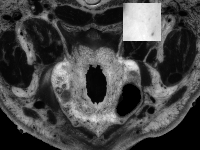
\includegraphics[width=\textwidth]{statistical_normals/lk/3d/images/occluded-example}
        \caption{}\label{fig:lk_occluded_example}
    \end{subfigure}
    \begin{subfigure}{0.47\columnwidth}
        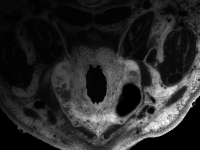
\includegraphics[width=\textwidth]{statistical_normals/lk/3d/images/biasfield-example}
        \caption{}\label{fig:lk_biasfield_example}
    \end{subfigure}
    \caption{Examples of images from the Visible Human 
             project~\cite{spitzer1996visiblehuman} 
             used in the LK experiments. (a) Artificially occluded image. The
             occlusion appears as the white square in the top right. (b) Image
             with simulated bias field.}
\label{fig:lk_affine_examples}
\end{figure}
%%%%%%%%%%%%%%%%%%%%%%%%%%%%%%%%%%%%%%%%
For the LK experiments, the data used was from the Visible Human
project~\cite{spitzer1996visiblehuman}. 
This data has an image structure that differs from
other common 3D image sources such as MR images. Each voxel in an image is
formed from physical slices that were taken from the body of a cadaver.
Therefore, the gradient information across the $x, y$ plane is incredibly rich
as it represents a true 2D-image. However, the 3D nature of the data is still
maintained as each image along the $z$-axis represents another slice acquired
from the body.

In all experiments an affine motion model was used and performance was measured
within an extension of the evaluation framework proposed 
in~\cite{tzimiropoulos2011robust}.
We used the Oral section from the Visible Human data 
set~\cite{spitzer1996visiblehuman} as
the target image. We selected 10 different regions of interest and parametrised
the regions as a set of points representing the bounding cube of the region.
These points were then perturbed using Gaussian noise of standard deviation
$\sigma$. Using the affine warp defined between the original and perturbed
points, we generate a distorted image. Then, given a warp estimate, we compute
the new template points and calculate the root mean square error (RMSE) between
the estimated and correct locations. The performance metric used to assess the
algorithms is the average convergence rate for each fixed $\sigma = [1, 10]$,
over each of the 10 regions of interest. An algorithm was considered to have
converged if it had a final RMSE of less than $2.0$ pixels after 30 iterations.
For each template, 100 convergence tests were performed. Each image was smoothed
using Gaussian smoothing with $\sigma = 2.0$ and kernel size $5\times5\times5$,
before the calculation of derivatives. All algorithms were implemented using the
inverse compositional form.

To provide a competitive assessment of our similarity measures, we extended
recent state-of-the-art 2D algorithms for use with 3D images. We concentrated on
algorithms that aim to provide robustness against outliers, particularly in the
form of intensity inhomogeneities. Therefore, we provide comparisons against the
enhanced correlation coefficient (ECC)~\cite{evangelidis2008parametric} 
and the Fourier LK
algorithm with Gabor filter banks (GaborFourier)~\cite{lucey2013fourier}. As a
baseline, we also compare against the standard LK algorithm and the iteratively
re-weighted least squares algorithm (IRLS) also proposed by
\citet{baker2005lk20yearsonpart5}.

We also compare against the most related technique that utilises the cosine
squared measure (CosineSquared)~\cite{haber2006intensity}. Our implementation of
CosineSquared is equivalent to the Gauss-Newton methodology described
within~\cite{haber2006intensity}.
%%%%%%%%%%%%%%%%%%%%%%%%%%%%%%%%%%%%%%%%%%%%%%%%%%%%%%%%%%%%%%%%%%%%%%%%%%%%%%%%
\paragraph{Experiments Without Corruption}\label{subsec:lk_results_nocorruption}
%%%%%%%%%%%%%%%%%%%%%%%%%%%%%%%%%%%%%%%%%%%%%%%%%%%%%%%%%%%%%%%%%%%%%%%%%%%%%%%%
In this subsection, we present our performance evaluation results obtained
without applying any corruption to the 3D images. We compared the performance of
the inverse-compositional LK algorithm (IC) with both forms of our algorithm,
InnerProduct and Spherical and the related method CosineSquared. This experiment
is designed as a baseline that presents the performance of robust measures in
data that is known to contain no outliers.

As \cref{fig:lk_results_nocorruption} shows, the IC algorithm outperforms
the other methods for this experiment. This result is unsurprising, as the
distorted image is generated directly from the original image without any
outliers. Since both of our proposed methods discard information in the form of
the gradient magnitude, they inevitably perform worse than the LK algorithm.
However, the difference between our two algorithms is negligible, which is
expected given that they both discard the same amount of information. The larger
deformations significantly decrease the performance of the CosineSquared
algorithm. This is likely due to the bias created by squaring the inner product
of the images.
%%%%%%%%%%%%%%%%%%%%%%%%%%%%%%%%%%%%%%%%%%%%%%%%%%%%%%%%%%%%%%%%%%%%%%%%%%%%%%%%
\paragraph{Experiments With Corruption}\label{subsec:lk_results_corrupted}
%%%%%%%%%%%%%%%%%%%%%%%%%%%%%%%%%%%%%%%%%%%%%%%%%%%%%%%%%%%%%%%%%%%%%%%%%%%%%%%%
In this subsection, we present three separate experiments: images with a
simulated bias field, with an occlusion and with an occlusion and a simulated
bias field. The bias field was generated as described in
\cref{subsubsec:bias_fields} and an example is shown in
\cref{fig:lk_biasfield_example}. Occluded sections were created
synthetically by randomly placing image sections taken from another random area
of the body, and putting them into every slice of the 3D image, as shown in
\cref{fig:lk_occluded_example}.

\cref{fig:lk_results_biasfield} shows that our proposed techniques are
competitive with the state-of-the-art for bias field corruption. The LK and IRLS
algorithms are not able to cope with the intensity variation caused by the bias
field. GaborFourier copes reasonably well with this type of corruption due to
the illumination invariant properties described in~\cite{lucey2013fourier}. ECC
performs very well, which is unsurprising as the enhanced correlation
coefficient performs a normalisation of the image pixels, which reduces the
effect of the bias field. The CosineSquared algorithm performs well for smaller
deviations, but quickly diminishes in performance.

\cref{fig:lk_results_occlusion} shows that our proposed similarity
measures are also the most robust to occlusions. IRLS performs better under
these situations as it is able to discard some of the outliers that bias the
alignment. The normalisation step in ECC has no benefit in suppressing this sort
of bias, and so it performs very similarly to the non-robust IC algorithm.
GaborFourier still performs well as the Gabor filter banks suppress the
contribution of the outliers. The CosineSquared performs well under smaller
deformations but is heavily biased under large deformations as the squaring of
the cosine fails to suppress the contribution of the occlusions.

Finally, in \cref{fig:lk_results_occlusion_biasfield} we see that even
under occlusion and global illumination variation, our proposed measures perform
with relatively high accuracy. This is a challenging experiment which
demonstrates the power of our proposed similarity measure. Despite the large
amount of outliers, our proposed measures are still able to perform accurate
alignment with a higher success rate than any of the other algorithms
considered.
%%%%%%%%%%%%%%%%%%%%%%%%%%%%%%%%%%%%%%%%
\begin{figure*}
    \centering
    \begin{subfigure}{0.52\textwidth}
        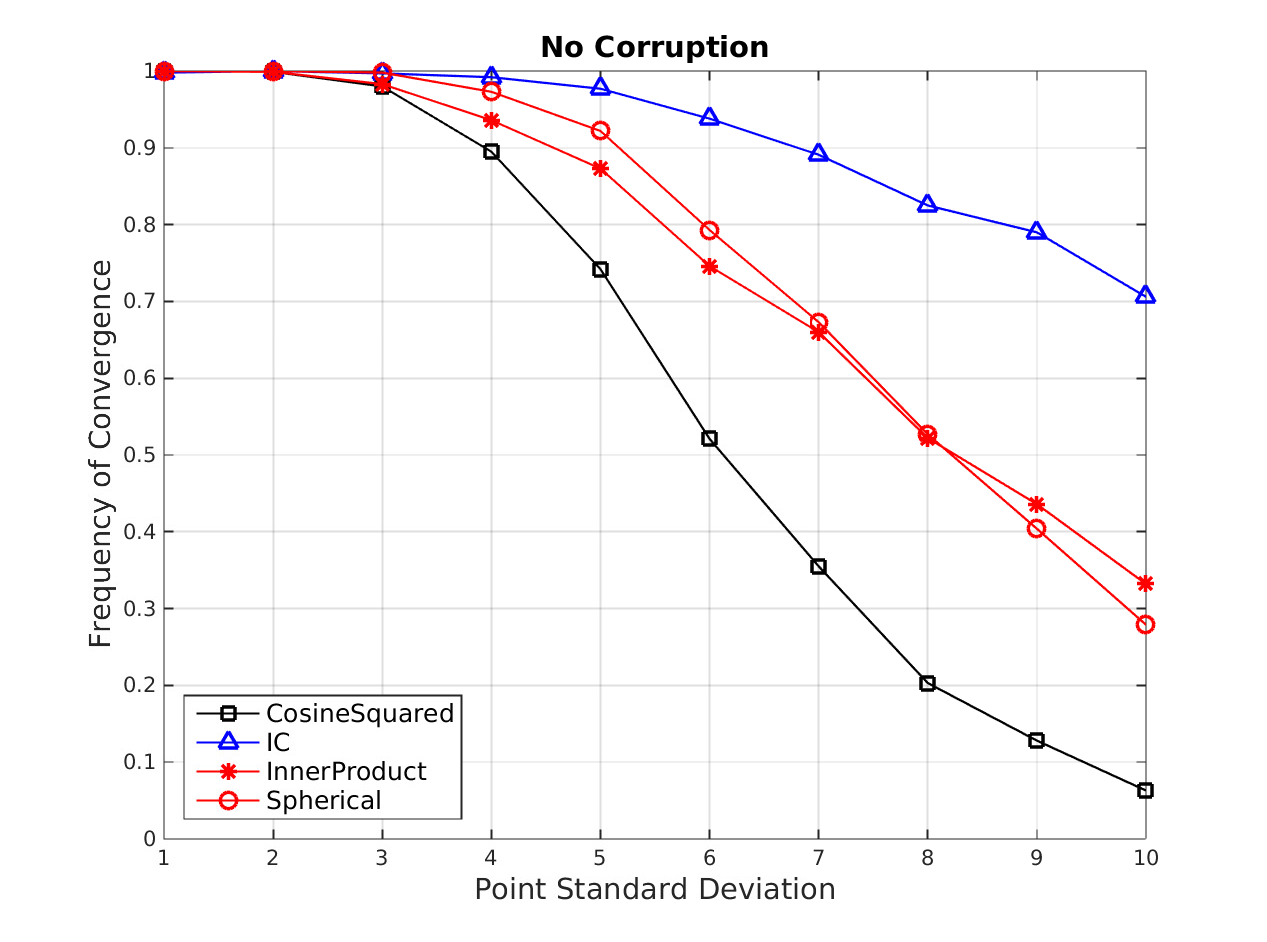
\includegraphics[width=\textwidth]{statistical_normals/lk/3d/images/NoCorruption_Smoothing_2-crop}
        \caption{}\label{fig:lk_results_nocorruption}
    \end{subfigure} \hspace*{-1cm}
    \begin{subfigure}{0.52\textwidth}
        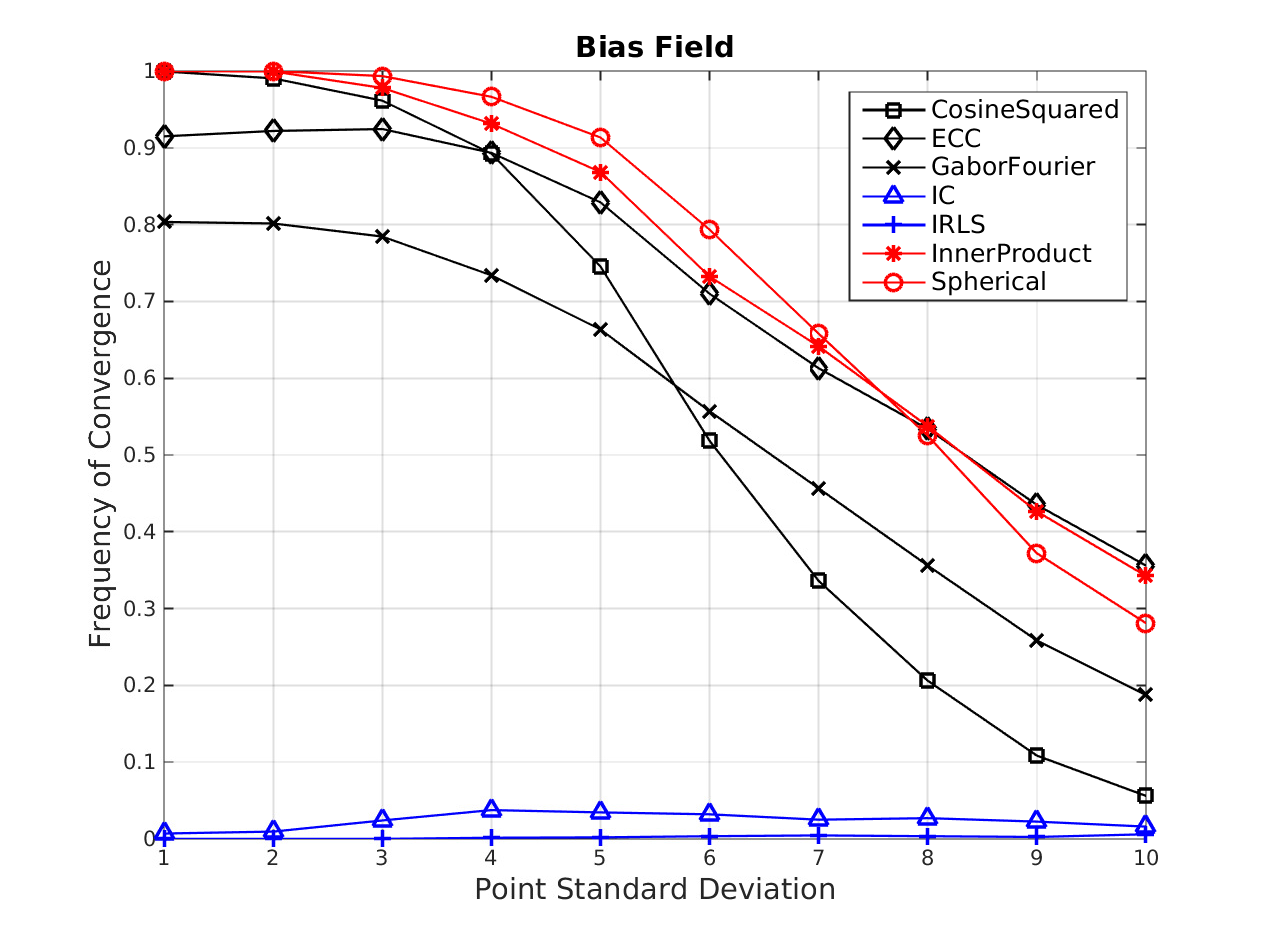
\includegraphics[width=\textwidth]{statistical_normals/lk/3d/images/BiasField_Smoothing_2-crop}
        \caption{}\label{fig:lk_results_biasfield}
    \end{subfigure} \\
    \begin{subfigure}{0.52\textwidth}
        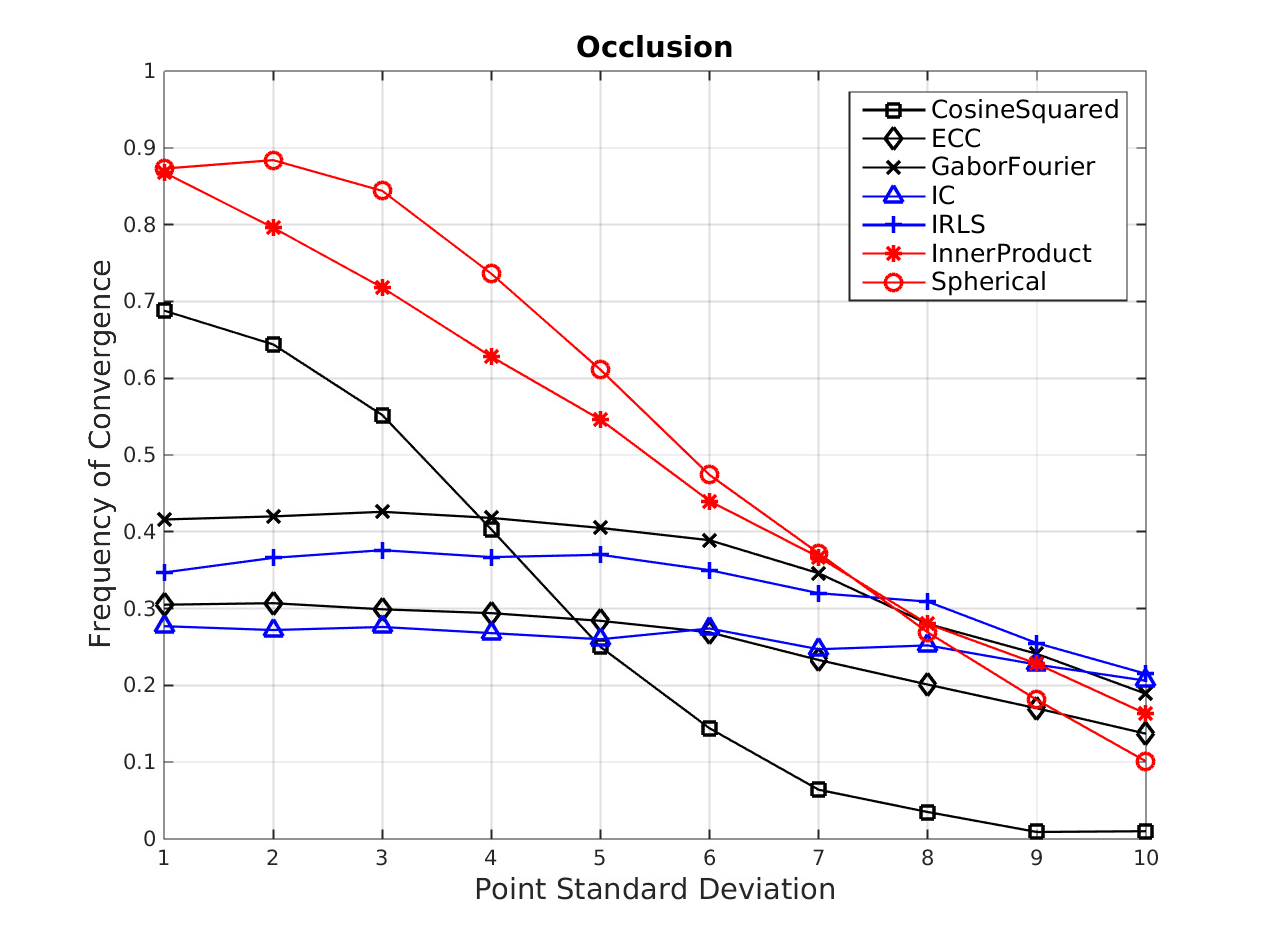
\includegraphics[width=\textwidth]{statistical_normals/lk/3d/images/Occlusion_Smoothing_2-crop}
        \caption{}\label{fig:lk_results_occlusion}
    \end{subfigure} \hspace*{-1cm}
    \begin{subfigure}{0.52\textwidth}
        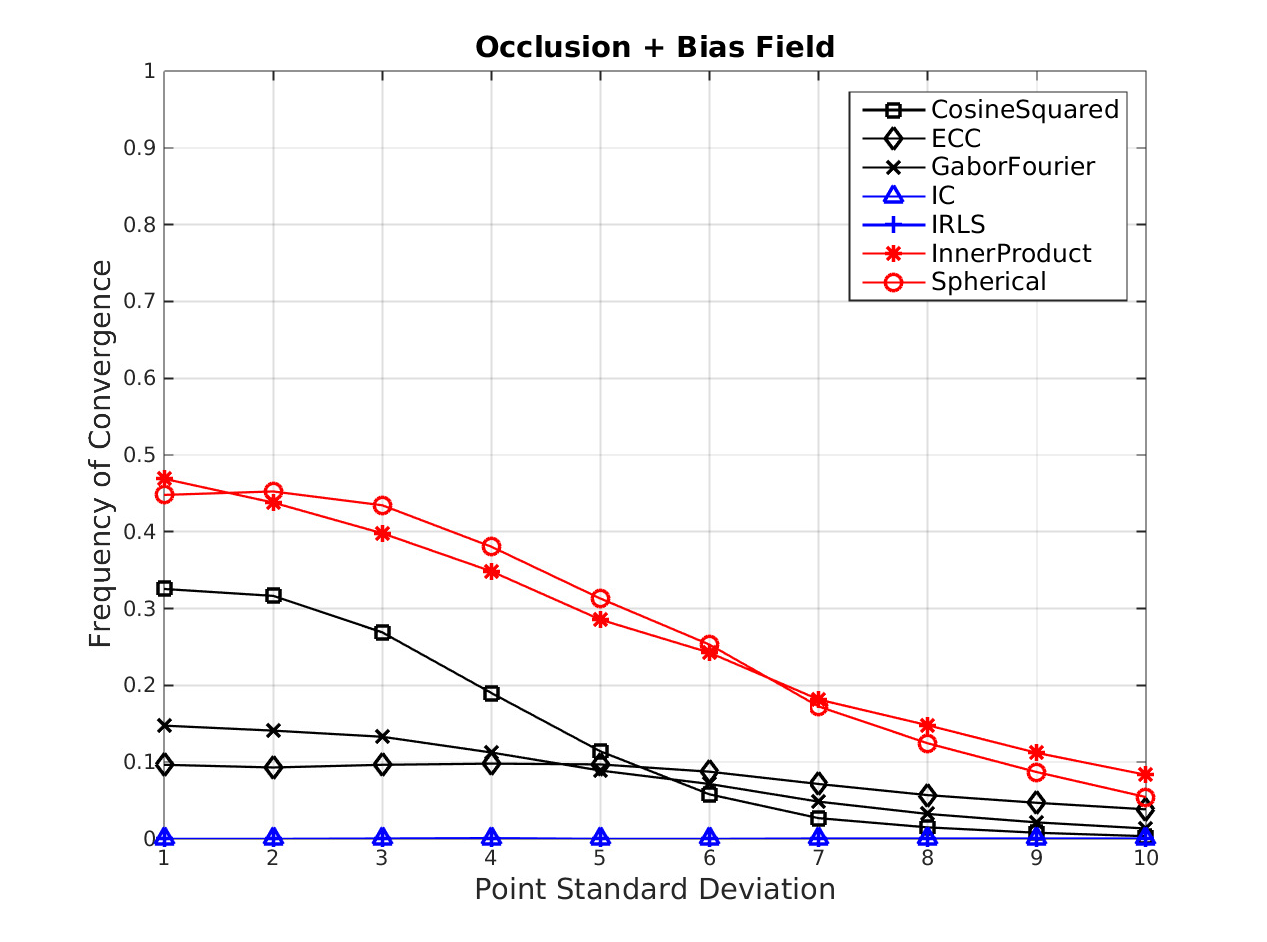
\includegraphics[width=\textwidth]{statistical_normals/lk/3d/images/Occlusion_BiasField_Smoothing_2-crop}
        \caption{}\label{fig:lk_results_occlusion_biasfield}
    \end{subfigure}
    \caption{Average frequency of convergence vs Point standard deviation for 
             the Visible Human data set. (a) Simulated Bias Field (b) Occlusions
             (c) Occlusions + Bias Field. CosineSquared: black-$\square$. ECC:\@
             black-$\diamond$. GaborFourier: black-x. IC:\@ blue-x. IRLS:\@
             blue-+. InnerProduct: red-*. Spherical: red-o}
\label{fig:lk_results_corrupted}
\end{figure*}
%%%%%%%%%%%%%%%%%%%%%%%%%%%%%%%%%%%%%%%%
